% MCDS Capstone Progress Document
% Kyle Dotterrer
% 4 October, 2021

%% ==================================================================
%% BOILERPLATE
%% ==================================================================

\documentclass{vldb}

\newcommand{\paperTitle}{JIT Compilation for User-Defined Functions\\ 
    \large Capstone Fall Progress Report\\
    \today}
\newcommand{\paperKeywords}{}
\newcommand{\paperAuthors}{}

\setlength{\paperheight}{11in}
\setlength{\paperwidth}{8.5in}

\usepackage[
            bookmarks=true,
            bookmarksopen=true,
            pdfhighlight=/I,
            pdfpagemode=UseOutlines,
            linkcolor=blue,
            pdfborder={ 0 0 0 },
            pageanchor=false]{hyperref}
\hypersetup{
    pdfauthor = {\paperAuthors},
    pdftitle = {\paperTitle},
    pdfkeywords = {\paperKeywords},
    pdfborder={ 0 0 0 }
}

\usepackage{amsmath}
\usepackage{amssymb}
\usepackage{times}
\usepackage{boxedminipage}
\usepackage{xspace}
\usepackage{array}
\usepackage{epsfig}
\usepackage{calc}
\usepackage{multirow}
\usepackage{rotating}
\usepackage{enumitem}
\usepackage[usenames,dvipsnames]{color}
\usepackage{tabularx}
\usepackage{tikz}
\usepackage{wasysym }
\usepackage[hyphenbreaks]{breakurl}
\usepackage{xcolor}
\usepackage[font={small}]{caption}
\usepackage{alltt}
\usepackage{setspace}
\usepackage{wrapfig}
\usepackage{etoolbox}

% Font selection
\usepackage[final]{microtype}
\usepackage[scaled]{inconsolata}
\usepackage[T1]{fontenc}
\usepackage{graphicx}
\usepackage{soul}
\usepackage{pifont}

% Other misc. things
\usepackage{float}
\usepackage{bookmark}
\usepackage{amsmath,amsfonts,amssymb}
\usepackage{latexsym}
\usepackage{multirow}
\usepackage{emptypage}
\usepackage{booktabs}
\usepackage{enumerate}
\usepackage{braket}
\usepackage{balance}

\usepackage[newfloat]{minted}

\definecolor{commentgray}{rgb}{0.2,0.2,0.2}
\definecolor{bggray}{rgb}{0.98,0.98,0.98}

\setminted{
  bgcolor=white,
  numberblanklines=false,
  frame=single,
  numbers=left,
  tabsize=2,
  xleftmargin=1.8em,
  xrightmargin=0.5em
}


%% ==================================================================
%% MACROS
%% ==================================================================

\newcommand{\subparagraph}{}

\newcommand{\sysname}{NoisePage\xspace}

% Framework Components
\newcommand{\dbTranslator}{Translator\xspace}
\newcommand{\dbCompiler}{Compiler\xspace}
\newcommand{\dbPlanner}{planner\xspace}
\newcommand{\dbInterpreter}{interpreter\xspace}
\newcommand{\dbAnalyzer}{analyzer\xspace}
\newcommand{\dbPCQ}{PCQ\xspace}
\newcommand{\dbAQP}{AQP\xspace}
\newcommand{\dbHook}{hook\xspace}
\newcommand{\dbHooks}{hooks\xspace}

\newcommand{\dbSQL}[1]{\texttt{\textbf{#1}}\xspace}
\newcommand{\dbTable}[1]{\texttt{\MakeUppercase{#1}}\xspace}
\newcommand{\dbColumn}[1]{\texttt{col#1}\xspace}
\newcommand{\dbRawColumn}[1]{\texttt{#1}\xspace}
\newcommand{\dbConfig}[1]{\textsf{#1}\xspace}

\newcommand{\dbmsOracle}{Oracle\xspace}
\newcommand{\dbmsDBTwo}{DB2\xspace}
\newcommand{\dbmsTeradata}{Teradata\xspace}
\newcommand{\dbmsHANA}{HANA\xspace}
\newcommand{\dbmsMSSQL}{SQL Server\xspace}
\newcommand{\dbmsMySQL}{MySQL\xspace}
\newcommand{\dbmsPostgres}{PostgreSQL\xspace}
\newcommand{\dbmsMemSQL}{MemSQL\xspace}
\newcommand{\dbmsHyper}{HyPer\xspace}
\newcommand{\dbmsVector}{Vector\xspace}

\newcommand{\tplType}[1]{\texttt{#1}\xspace}
\newcommand{\tpl}{\texttt{TPL}\xspace}
\newcommand{\tbc}{\texttt{TBC}\xspace}
\newcommand{\dbCode}[1]{{\sffamily\small \textbf{#1}}\xspace}

\newcommand{\tidlist}{\texttt{TupleIdList}\xspace}
\newcommand{\tidlists}{\texttt{TupleIdLists}\xspace}

%% ==================================================================
%% PAPER CONTENT
%% ==================================================================

\begin{document}

\title{\paperTitle}

\numberofauthors{2}
\author{
    \alignauthor Kyle Dotterrer, Andrew Pavlo\\
    \affaddr{Carnegie Mellon University}\\
    \email 
        \{\href{mailto:kdottere@cs.cmu.edu}{kdottere},
        \href{mailto:pavlo@cs.cmu.edu}{pavlo}\}@cs.cmu.edu\\
}

% Remove the space for the copyright box for VLDB
\makeatletter
\def\@copyrightspace{\relax}
\makeatother

\maketitle

%% ==================================================================
%% INTRODUCTION
%% ==================================================================

\section{Introduction}

This document provides a description of the progress made this semester towards achieving the goals of this capstone. Section 2 provides an overview of the domain and a high-level description of the problem we are attempting to solve. Next, in section 3, we provide further details regarding the aspects of the problem we have addressed so far this semester. Section 4 breaks the problem down into actionable points and describes how we are making progress towards achieving each of these. In Section 5 we present preliminary results. Section 6 provides a status update specifically targeting the feedback received during submission of the Fall Completion Plan. In Section 7 we reflect on areas of improvement for the project. We conclude in Section 8 by describing our next steps.

%% ==================================================================
%% MOTIVATION
%% ==================================================================

\section{Motivation}

User-defined functions (UDFs) are a powerful tool for encapsulating complex application logic that may subsequently be embedded into SQL queries. Consider a scenario in which we would like to write a query that computes the "reward level" for each customer in a table of retail transactions based on the total amount spent by each customer. Expressing such a query in pure SQL is certainly possible, but non-trivial. In contrast, with the help of SQL's procedural extensions, the definition of a UDF that implements this logic is straightforward, as shown in figure~\ref{fig:cust_level_def}.

\begin{listing}[H]
    \begin{minted}[frame=lines]{plpgsql}
CREATE FUNCTION cust_level(ckey int)
    RETURNS CHAR(10) AS $$
    DECLARE total FLOAT;
    DECLARE level CHAR(10);
BEGIN
    total = (SELECT SUM(o_totalprice) 
        FROM orders WHERE o_custkey=ckey);
    IF (total > 1000000)
        level = 'Platinum';
    ELSE
        level = 'Regular';
    END IF;
    RETURN level;
END 
$$ LANGUAGE PLPGSQL;
    \end{minted}
    \caption{The definition of UDF \dbCode{cust\_level}.}
    \label{fig:cust_level_def}
\end{listing}

Once the UDF is defined, we can then use the UDF in subsequent queries to efficiently express high-level application logic. A query that invokes the UDF \dbCode{cust\_level} is shown in figure~\ref{fig:cust_level_call}.
    
\begin{listing}[H]
    \begin{minted}[frame=lines]{plpgsql}
SELECT c_custkey, cust_level(c_custkey)
    FROM customer;
    \end{minted}
    \caption{The invocation of UDF \dbCode{cust\_level}.}
    \label{fig:cust_level_call}
\end{listing}

Although they offer a practical complement to SQL, their use in production database environments is often limited because of their associated performance costs \cite{froid, apfel}. For instance, a recent study from a team at Microsoft finds that expressing the same logic in SQL and SQL with procedural extensions may lead to an orders-of-magnitude increase in query runtime - from milliseconds to over thirteen hours \cite{froid}.

In this project, we evaluate the efficacy of methods intended to address the performance limitations of UDFs in the context of relational database management systems (DBMSs). We compare the performance of an existing, state-of-the-art technique, UDF inlining, with our own novel strategy that executes UDFs as native code via JIT-compilation. Our evaluation efforts are ongoing.

%% ==================================================================
%% PROBLEM STATEMENT
%% ==================================================================

\section{Problem Statement}

During the first half of this semester, we focused our efforts on designing and implementing benchmarks for the UDF performance optimization techniques under consideration. 

With the majority of the engineering effort required to implement our novel approach to UDF JIT-compilation completed, we are now able to turn our attention to answering our research questions: 

\begin{itemize}
    \item \textit{Which of the approaches to UDF runtime optimization performs best?}
    \item \textit{If there is not a single, dominant technique that outperforms the others under all conditions, under which sets of conditions does each technique excel?}
    \item \textit{Why does one technique outperform another under a particular set of conditions?}
\end{itemize}

We aim to answer these questions empirically - by performing a series of experiments in which we compare the performance of UDFs executed with our novel approach to UDF JIT-compilation against those produced by systems that perform UDF-inlining \cite{apfel, froid}. We partition this empirical evaluation into the following subproblems:

\begin{itemize}
    \item \textbf{Identification of Benchmarks} The first step in our evaluation is to determine the set of benchmarks we intend to run. This decision drives the remainder of the process.
    \item \textbf{Preparation of Evaluated Functions and Queries} Once the benchmarks are decided upon, we must prepare the individual functions (UDFs) and their invoking queries for input to the benchmarking process. We intend to run all benchmarks in the context of the NoisePage research DBMS \cite{noisepage}, so preparation of functions and queries from the output of other systems requires manual implementation of query plans in the NoisePage domain specific language (DSL) \tpl.
    \item \textbf{Preparation of Benchmarking Infrastructure} Performance benchmarks for high-performance systems require a high-degree of automation to support replicability. This allows us to run individual benchmarks over many iterations, across multiple software and hardware environments so that we may be assured of the generality of our results. In this context, benchmarking infrastructure refers to the set of scripts that we utilize to automate the benchmarking process.
    \item \textbf{Execution of Benchmarks} Once the benchmarking infrastructure is complete and tested, we can use it to run the benchmarks themselves and collect results.
    \item \textbf{Communication of Benchmark Results} Finally, once we have the benchmark results, we must organize and communicate them in a way that allows us to draw meaningful conclusions.
\end{itemize}

Our progress towards each of these specific sub-problems is described in the \textit{Project Plan} section below.

%% ==================================================================
%% PROJECT PLAN
%% ==================================================================

\section{Project Plan}

During the first half of the semester, we made progress towards each of the sub-problems identified above. In this section, we provide further details describing the steps we have taken towards achieving our objective.

\subsection{Identification of Benchmarks} 

During the first part of this semester, we identified the benchmarks we intend to run to evaluate UDF optimization techniques. These include the following:

\begin{itemize}
    \item \textbf{Synthetic Benchmark \textit{Call}} This manually constructed benchmark evaluates the overhead of a function call in our implementation of UDF JIT-compilation. This benchmark is adapted from prior work by Nayak \cite{tanuj}.
    \item \textbf{Synthetic Benchmark \textit{Loop}} This manually-constructed benchmark evaluates the computational efficiency of our implementation of UDF JIT-compilation. This benchmark is adapted from prior work by Nayak \cite{tanuj}.
    \item \textbf{Select Functions from SQL ProcBench}. SQL ProcBench \cite{procbench} is a new DBMS benchmark specifically designed to emulate the types of UDF workloads found in production environments. We select a subset of functions from this benchmark for our evaluation. Functions were selected based on the ability of each framework under consideration to properly handle the constructs used in the functions and their associated invoking queries. A complete description of the reason each function was selected along with the function definitions themselves can be found at \cite{udf-jit}.
\end{itemize}

\subsection{Preparation of Evaluated Functions and Queries} 

In addition to compiling and executing UDFs on NoisePage, we require outputs from the UDF inling frameworks \textit{Froid} \cite{froid} and \textit{Apfel} \cite{apfel} in order to perform our evaluation. These represent state-of-the-art approaches to the problem of UDF performance optimization, but they accomplish this in a way that is different from our JIT-compilation technique.

All inlined query plans from Microsoft SQL Server have been gathered and are available at \cite{udf-jit}. We have collected the inlined versions of all but two of the SQL ProcBench functions from the Apfel framework via its web interface, and we are working with the authors of the framework to address the issues that inhibit compilation of the remaining functions.

What remains to be done for the queries produced by these two frameworks is manual implementation of the query plans in NoisePage's internal DSL - \tpl - that will allow us to execute them on our research platform. This will be the primary focus of the remainder of the semester.

\subsection{Preparation of Benchmarking Infrastructure} 

We have written a collection of scripts that automate all aspects of the benchmarking process, from creating and loading tables to executing the benchmarks themselves and recording results. All of these scripts are available at \cite{udf-jit}. 

\subsection{Execution of Benchmarks} 

The collection of benchmarking scripts described above removes much of the manual effort involved in running benchmarks. By combining hardware owned by the CMU Database Group with access to AWS EC2 on-demand instances, we have a variety of hardware environments for benchmarking.

\subsection{Communication of Benchmark Results} 

We provide preliminary results of our benchmarks in the following section. These graphics and figures do not necessarily reflect the versions that will appear in our final report, but they do give some indication of both the strengths and weaknesses of our approach.

%% ==================================================================
%% PROGRESS
%% ==================================================================

\section{Progress}

In this section, we present initial results from our evaluation. The first aspect of our implementation we intend to evaluate is the overhead imposed by individual function calls. While this does not reflect performance improvements or degregations on production workloads, it does allow us to quickly evaluate the viability of our approach to UDF optimization via JIT compilation.

In order to measure the runtime overhead imposed by an individual function call, we design a simple synthetic benchmark \textit{Call}. This benchmark consists of three queries:

\begin{itemize}
    \item A baseline query that simply performs a sequential scan over a single integer column of a table. This query is shown in listing~\ref{list:udf_call_baseline}. 
    \item A query that invokes the UDF \dbCode{addOne} to increment this integer column by the constant value one. The definition of \dbCode{addOne} is shown in listing~\ref{list:udf_call_functiondef} and the associated invocation is shown in listing~\ref{list:udf_call_function}.
    \item A query that represents a "perfectly-inlined" version of the call to UDf \dbCode{addOne}. In this query, the logic to increment the integer column is completely inlined into the top-level query, eliding the function call entirely. This query is shown in figure~\ref{list:udf_call_inlined}.
\end{itemize}

\begin{listing}
    \begin{minted}[frame=lines]{sql}
SELECT x FROM integers;
    \end{minted}
    \caption{The baseline query for evaluating the overhead of a UDF call.}
    \label{list:udf_call_baseline}
\end{listing}

\begin{listing}
    \begin{minted}[frame=lines]{plpgsql}
CREATE FUNCTION addOne(x INTEGER) 
    RETURNS INTEGER AS $$
BEGIN
    RETURN x + 1;
END
$$ LANGUAGE PLPGSQL;
    \end{minted}
    \caption{The definition of UDF \dbCode{addOne}.}
    \label{list:udf_call_functiondef}
\end{listing}

\begin{listing}
    \begin{minted}[frame=lines]{sql}
SELECT x, addOne(x) FROM integers;
    \end{minted}
    \caption{The inlined query for evaluating the overhead of a UDF call.}
    \label{list:udf_call_function}
\end{listing}

\begin{listing}
    \begin{minted}[frame=lines]{sql}
SELECT x, x + 1 FROM integers;
    \end{minted}
    \caption{The inlined query for evaluating the overhead of a UDF call.}
    \label{list:udf_call_inlined}
\end{listing}

We run this performance benchmark on two systems: PostgreSQL 12 and NoisePage. Here, PostgreSQL serves as a baseline against which we compare our implementation. PostgreSQL implements UDF execution in a manner that incurs significant context-switching overhead \cite{apfel}. As a consequence of this, we expect to observe high function-call overhead in PostgreSQL. In contrast, the benchmark run on NoisePage uses our approach to UDF JIT-compilation that should avoid context switching overhead by virtue of the fact that all of the logic is expressed as a single program in our internal DSL. 

The results of this benchmark are shown in figure~\ref{fig:bench_pg_call} and figure~\ref{fig:bench_np_call}. The results demonstrate the expected trend: UDF execution in PostgreSQL is slower in absolute terms than UDF execution in NosiePage. More importantly, as the size of the table grows, the overall query runtime for PostgreSQL scales much more poorly that it does for NoisePage. This indicates that our implementation of UDF JIT-compilation does not incur large function call overhead, relative to the "optimal" inlined version of the query.

\begin{figure}[t!]
    \centering
    
\includegraphics[width=\columnwidth]{plots/pg_call_legend.pdf}
    \\
    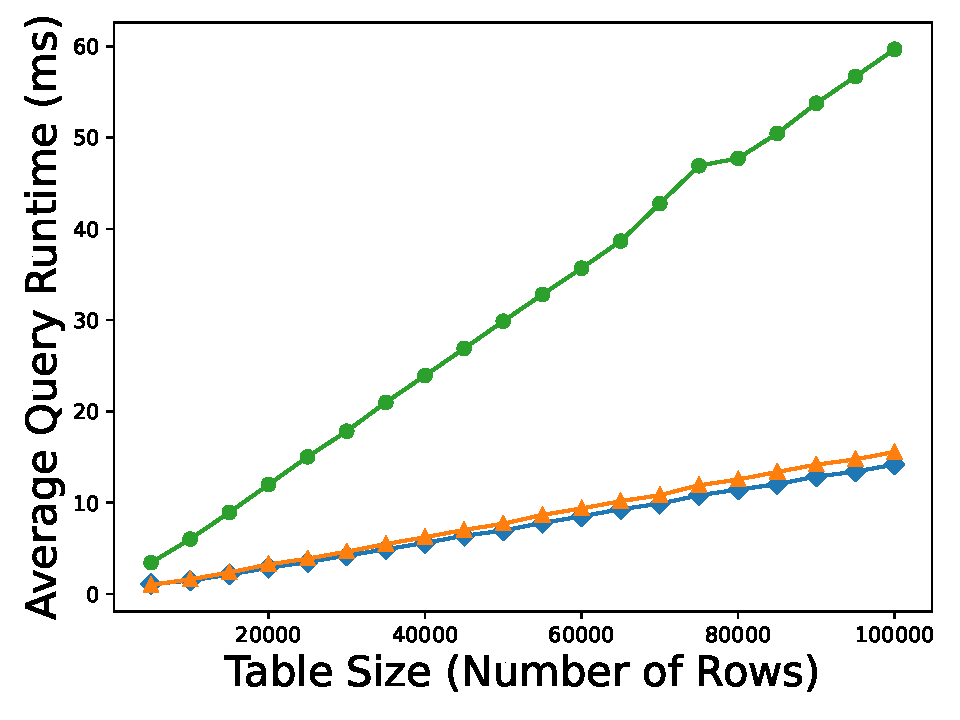
\includegraphics[width=\columnwidth]{plots/pg_call.pdf}
    \caption{
        \textbf{Function Call Overhead (PostgreSQL)} --
        Comparison among baseline query, inlined column increment, and column increment with a function call to UDF \dbCode{addOne} in PostgreSQL.
    }
    \label{fig:bench_pg_call}
\end{figure}

\begin{figure}[t!]
    \centering
    
\includegraphics[width=\columnwidth]{plots/np_call_legend.pdf}
    \\
    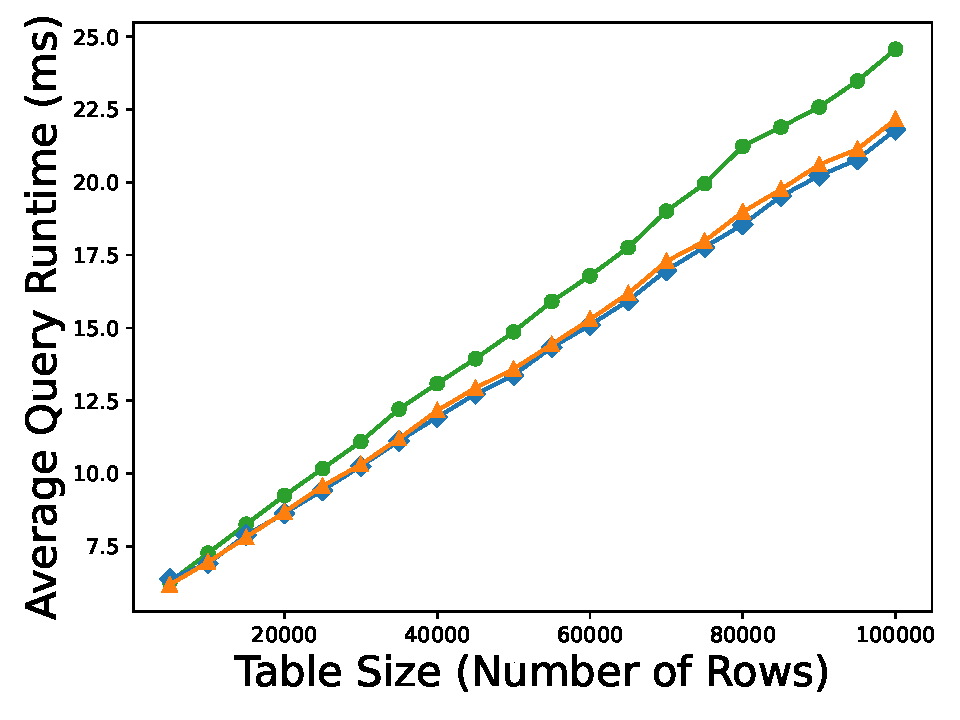
\includegraphics[width=\columnwidth]{plots/np_call.pdf}
    \caption{
        \textbf{Function Call Overhead (NoisePage)} --
        Comparison among baseline query, inlined column increment, and column increment with a function call to UDF \dbCode{addOne} in NoisePage.
    }
    \label{fig:bench_np_call}
\end{figure}

We construct a second benchmark, \textit{Loop}, to evaluate the viability of our approach to UDF JIT-compilation against the PostgreSQL baseline. In this benchmark, we evaluate the total runtime required for the UDF execution engine to execute a tight loop for a specified number of iterations. Like the previous benchmark, this benchmark does not serve as an indicator of performance on production workloads, but rather demonstrates the potential of our approach to remove software overheads via JIT-compilation of functions.

The definition of the \dbCode{busyLoop} function is provided in listing~\ref{list:udf_loop}. This function is invoked with arguments ranging from 10-100,000,000 specifying the number of iterations of the loop executed within the function's body. The results of the benchmark are shown in figure~\ref{fig:bench_loop}. We see that as the number of iterations grows by a factor of 10, increasing from 10,000,000 to 100,000,000, the total query runtime on PostgreSQL explodes as a result of the relatively-high overhead of individual iterations. In contrast, the growth in runtime for NoisePage is much more modest, suggesting that our approach to UDF JIT-compilation elides much of the overhead imposed by interpreter-based systems like PostgreSQL.

\begin{listing}
    \begin{minted}[frame=lines]{plpgsql}
CREATE FUNCTION busyLoop(x INTEGER) 
    RETURNS INTEGER AS $$
DECLARE
    c INTEGER := 0;
BEGIN
    WHILE c < x LOOP;
        c = c + 1;
    END LOOP;
    RETURN c;
END
$$ LANGUAGE PLPGSQL;
    \end{minted}
    \caption{The definition of UDF \dbCode{busyLoop}.}
    \label{list:udf_loop}
\end{listing}

\begin{figure}[t!]
    \centering
    
\includegraphics[width=\columnwidth]{plots/loop_legend.pdf}
    \\
    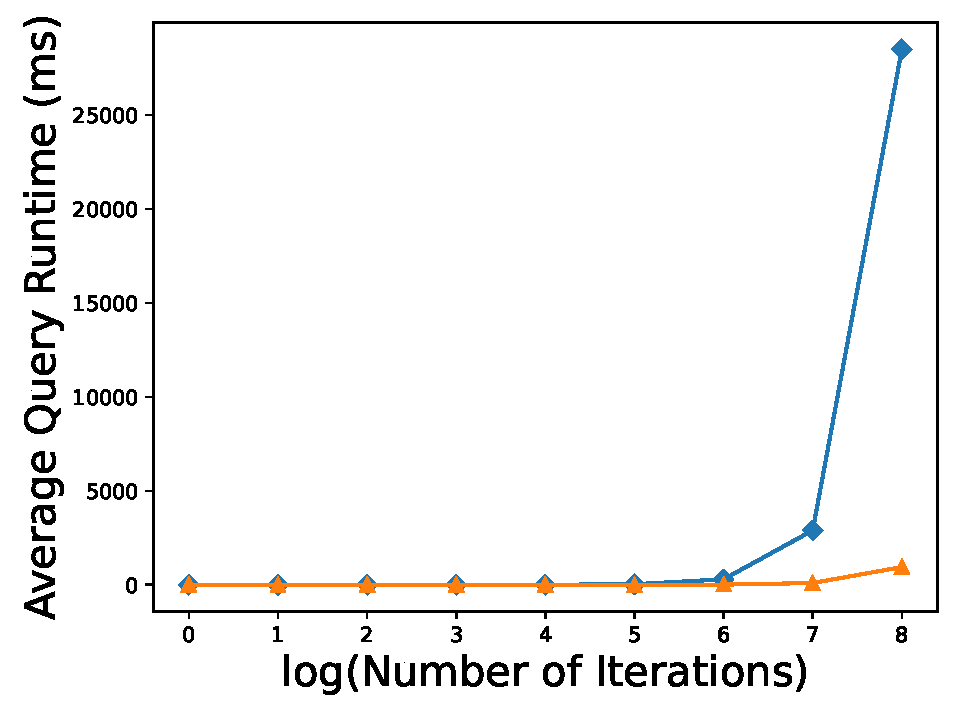
\includegraphics[width=\columnwidth]{plots/loop.pdf}
    \caption{
        \textbf{Function Call Scalability} --
        Comparison of the runtime required by PostgreSQL and NoisePage to execute the UDF \dbCode{busyLoop} for a specified number of iterations.
    }
    \label{fig:bench_loop}
\end{figure}

Finally, we perform an initial evaluation on a selected functions from the SQL ProcBench \cite{procbench} benchmark. The performance evaluation is performed on the NoisePage system. Results from running this benchmark against PostgreSQL 12 are also included to provide a point of comparison. We note that, unlike the previous synthetic benchmarks, this benchmark reflects the complete end-to-end performance characteristics of the tested system, rather than the performance characteristics of the UDF execution subsystem in isolation. Results of this benchmark are shown in figure~\ref{fig:bench_procbench}.

\begin{figure}[t!]
    \centering
    
\includegraphics[width=\columnwidth]{plots/procbench_legend.pdf}
    \\
    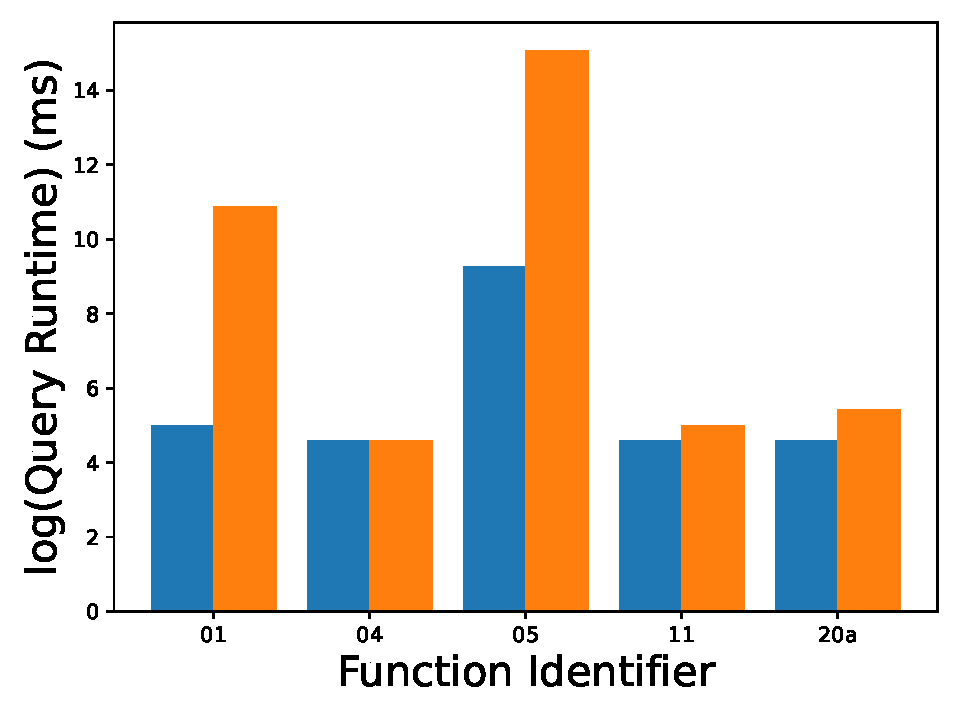
\includegraphics[width=\columnwidth]{plots/procbench.pdf}
    \caption{
        \textbf{End-to-End Benchmark Performance} --
        Comparison of query runtime on PostgreSQL and NoisePage during execution of select functions from the SQL ProcBench benchmark.
    }
    \label{fig:bench_procbench}
\end{figure}

Unlike the previous two benchmarks, the results of this benchmark are far from inspiring. NoisePage achieves runtimes similar to PostgreSQL for several of the functions (function identifiers \dbCode{04}, \dbCode{11}, and \dbCode{20a}), but far underperforms PostgreSQL on the remaining functions (function identifiers \dbCode{01} and \dbCode{05}). The distinction between these two sets of functions is that functions in the former group does not interact heavily with the NoisePage storage subsystem, while functions in the latter group do. As a specific example, the definition of the UDF with function identifier \dbCode{05} is shown in listing~\ref{list:udf_procbench_05}. The logic in this function is not complex, but it does involve two aggregations over the result of a three-way \dbCode{JOIN} on three relatively-large tables, implying that most of the work for this query occurs in the storage subsystem as tables are scanned and the \dbCode{JOIN} predicates are applied. The NoisePage storage subsystem has several design deficiencies that render this bottleneck unavoidable.

NoisePage's poor performance on these benchmark functions does not directly influence our ability to complete our evaluation. From the beginning of this project, we have planned to conduct our evaluation within the context of a single research platform in order to neutralize precisely these types of differences among database systems. However, it might preclude our ability to produce results suitable for publication.

\begin{listing}
    \begin{minted}[frame=lines]{plpgsql}
CREATE OR REPLACE FUNCTION morningToEveRatio(dep INT) 
    RETURNS INT AS $$
DECLARE
    morningSale INT;
    eveningSale INT;
    totalSale INT;
BEGIN
    morningSale := (SELECT COUNT(*)
        FROM web_sales, time_dim, customer_demographics
        WHERE ws_sold_time_sk = t_time_sk 
            AND ws_bill_customer_sk = cd_demo_sk
            AND t_hour >= 8 AND t_hour <= 9
            AND cd_dep_count = dep);

    eveningSale := (SELECT COUNT(*)
        FROM web_sales, time_dim, customer_demographics 
        WHERE ws_sold_time_sk = t_time_sk 
            AND ws_bill_customer_sk = cd_demo_sk
            AND t_hour >= 19 AND t_hour <= 20
            AND cd_dep_count = dep);

    totalSale := morningSale + eveningSale;
    RETURN totalSale;
END; 
$$ LANGUAGE PLPGSQL;
    \end{minted}
    \caption{The definition of ProcBench UDF \dbCode{05}.}
    \label{list:udf_procbench_05}
\end{listing}

%% ==================================================================
%% PROGRESS ON FEEDBACK
%% ==================================================================

\section{Progress on Feedback}

The primary point of feedback we received from the Fall update presentation was our failure to include a detailed timeline for our remaining project goals, specifically our publication plans. We address this shortcoming in the \textit{Next Steps} section below.

%% ==================================================================
%% SELF-APPRAISAL
%% ==================================================================

\section{Self-Appraisal}

The performance bottleneck in the NoisePage storage subsystem is well-known to developers within the CMU Database Group - this is a problem that we have known about for a long time but has gone un-addressed because it has not directly hindered our ability to conduct research. However, as noted above, this limitation may indeed hinder our ability to pursue our original publication plans.

This is an issue that has only come to light within the past week while running our first round of benchmarks from SQL ProcBench. We should have foreseen this issue long before reaching this point in the project and formulated a plan to either address it or avoid it entirely. 

%% ==================================================================
%% NEXT STEPS
%% ==================================================================

\section{Next Steps}

Our plan for completing our project is described by the timeline below.

\begin{center}
    \begin{tabular}{ |c|l| } 
        \hline
        \textbf{Date} & \textbf{Milestone} \\ 
        \hline
        08 October 2021 & Remaining Functions from \textit{Apfel} Compiled \\
        \hline
        15 October 2021 & 3/6 Inlined Functions from \textit{Apfel} Programmed \\
        \hline
        22 October 2021 & 6/6 Inlined Functions from \textit{Apfel} Programmed  \\
        \hline
        29 October 2021 & 3/6 Inlined Functions from \textit{Froid} Programmed \\
        \hline
        05 November 2021 & 6/6 Inlined Functions from \textit{Froid} Programmed \\
        \hline
        12 Novermber 2021 & Final Benchmarks Complete \\
        \hline
        21 November 2021 & Capstone Report Draft Submitted \\
        \hline
        06 December 2021 & Capstone Presentation \\
        \hline
        11 December 2021 & Capstone Final Report Submitted \\
        \hline
    \end{tabular}
\end{center}

In our Fall update presentation, we described our plans to pursue a publication as a result of this research. The viability of a publication is now in doubt as a result of the performance limitations of the NoisePage storage subsystem. Results acceptable for publication will likely require require further engineering effort that is outside the scopze of the capstone project. Discussions regarding the appropriate path forward with respect to publication are ongoing.

%% ==================================================================
%% BIBLIOGRAPHY
%% ==================================================================

% NOTE: Had to add this mysterious command to compile...
\newcommand{\newblock}{}

\clearpage
\bibliographystyle{abbrv}
\bibliography{progress}

\end{document}